
\begin{His}
Avant les décimaux, on utilisait les fractions. T'es tu demandé par exemple pourquoi les œufs sont vendus par 12 ?

Parce que c'est facile de partager une douzaine d'œufs en deux, mais aussi en trois, en quatre, en six.

Une fraction très utilisée était aussi la fraction sexagésimale (1/60). D'ailleurs on la trouve encore dans les minutes et les secondes: 
\begin{description}
\item[•] Une minute = 1/60 d’heure
\item[•] Une seconde = 1/60 de minute
\end{description}

60 est le plus petit nombres qui à le plus de diviseurs.

\vspace{0.4cm}
\begin{wrapfigure}[10]{r}{3.6cm}
\vspace{-7mm}
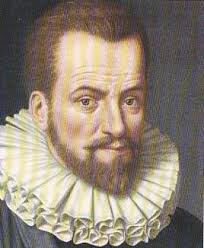
\includegraphics[scale=0.5]{image_chapitres/stevin.jpg}
\unnumberedcaption{Simon \textbf{Stevin}} 
\end{wrapfigure}
\textbf{Simon \textbf{Stevin}} est né à Bruges en 1548. Il a été employé de banque, ingénieur civil et militaire, professeur de mathématiques. C'est un homme très influent dans son pays et aussi un inventeur: il invente un char à voiles qui est capable de parcourir près de 80 km avec une trentaine de passagers en deux heures sur les plages de la mer du Nord de Scheveningen à Petten.

\vspace{0.2cm}
En 1585, il écrit "La Disme", d'abord publiée en flamand, \textbf{Stevin} lui-même la traduit en français.

\vspace{0.2cm}

\textit{Quelqu'un voyant la taille de ce livret, et la comparant à votre grandeur, mes très honorés  Seigneurs auxquels il est dédié, le trouvera sans doute absurde, mais s'il considère au contraire son utilité, il verra alors que sa taille n'a rien à voir avec son intérêt.}

\textit{Mais de quoi est-il question?  De quelque invention admirable?}
 
\textit{Non certes, mais d'une chose si simple qu'elle ne mérite quasi pas le nom d'invention, car de même que  l'homme rustique, et lourd, trouve parfois d'aventure quelque grand trésor, sans y avoir usé de science, c'est  ainsi que cette découverte est advenue. Pourtant si quelqu'un m'accuse de me  vanter de mon intelligence à cause de  mes explications, sans doute il démontre, soit qu'il est stupide  et incapable de savoir discerner les choses simples des ingénieuses, soit  qu'il soit envieux de la prospérité commune. Mais quoi qu'il en soit, son inutile calomnie ne doit pas faire oublier l'utilité de ce livret. Ainsi comme on ne reproche pas au marin qui a découvert une île inconnue, d'en vanter au roi les richesses comme les fruits, les minéraux précieux et les plaisantes contrées, on me permettra de parler librement de la grande utilité de cette invention. Oui je dis grande voire même plus grande qu'aucun d'entre vous ne s'y attend !}

\textit{Voilà donc que la matière dont il est question dans cette Disme (la première définition donnée peu après éclaircira ce nom) est le nombre.}

\textit{Il ne me sera pas nécessaire de rentrer dans les détails de son intérêt car vos multiples expériences professionnelles la rendent  assez claire.}

\textit{En effet, si je m'adresse à l'astrologue, il connait l'élévation de l'Équateur, et du Pôle, par le moyen de la table des déclinations du Soleil, il connait la vraie longitude et latitude des lieux mais il connait aussi la difficulté des multiplications, divisions en degrés, minutes et secondes …
Si je m'adresse au géomètre, il sait  que grâce à lui et sa science de nombreuses querelles et difficultés sont évitées. Des conflits éclateraient sans doute quotidiennement, à propos de la  surface des terres. En plus de cela,  il n'ignore pas (principalement celui auquel les affaires sont grandes) les ennuyeuses multiplications des Verges, Pieds, et souvent Doigts, l'un par l'autre, souvent sources d'erreurs, lésant l'un ou de l'autre des partis et parfois aussi conduisant à la ruine sa propre renommée. Beaucoup de précautions mais ceux qui maîtrisent alors les mesures sont rares et puissants.}

\vspace{0.2cm}

\textit{Ils maîtrisent les "nombres rompus " par exemple :}

\begin{description}
\item l'empan : Distance entre le pouce et l'un des quatre autres doigts . Il y a donc quatre valeurs différentes de l'empan
\item la coudée : c'est la longueur de l'avant-bras ( distance entre le coude et l'extrémité du majeur ) ; elle vaut 2 empans
\item la brasse : Ecart des bras aux poignets ou aux mains fermées . Elle vaut 8 empans et 4 coudées
\end{description}
\textit{Une pièce d'étoffe pouvait donc mesurer : 1 brasse, 3 coudées et 1 empan de long pour 3 coudées et 1 empan de large.
Difficile de calculer sa surface!}

\vspace{0.2cm}

La proposition de \textbf{Stevin}: Utiliser un système déjà bien maîtrisé pour les nombres entiers : \textbf{le système décimal}.

\vspace{0.2cm}


\hfill{D'après Christine \textbf{Paquet}, CPC. Académie de lyon}
\end{His}
